\documentclass[12pt,a4paper]{article}
\usepackage{amsmath,amssymb,amsthm}
\usepackage{makeidx,graphics}
\usepackage[dvips]{graphicx}
%\usepackage[latin1]{inputenc}
%\usepackage[portuguese]{babel}
\usepackage[utf8]{inputenc}
\usepackage{ae}
\usepackage{indentfirst}
\usepackage{amsbsy}
\usepackage{fancyhdr}
\usepackage{pstricks}
\usepackage[all]{xy}
\usepackage{wrapfig}
\usepackage[pdfstartview=FitH,backref,colorlinks,bookmarksnumbered,bookmarksopen,linktocpage,urlcolor=blue,
linkcolor=cyan]{hyperref}
\usepackage{bussproofs}
\usepackage{amsmath}
\usepackage{mathtools}
\usepackage{amsthm}
\usepackage{amsfonts}
\usepackage{amssymb}
\usepackage{wasysym}
\usepackage{amsbsy}
\usepackage{url}
%\usepackage{subfigure}
\usepackage{subcaption}
\usepackage{pgfplots}
\pgfplotsset{compat=newest}
\usepgfplotslibrary{fillbetween}

\usepackage{esint}

\newtheorem{definition}{Definição}
%\newtheorem{example}{Exemplo}
\newtheorem{lema}{Lema}
\newtheorem{teorema}{Teorema}
\newtheorem{corolario}{Corolário}
\newtheorem*{obs}{Observação}

\setlength{\topmargin}{-1.0in}
\setlength{\oddsidemargin}{0in}
\setlength{\evensidemargin}{0in}
\setlength{\textheight}{10.5in}
\setlength{\textwidth}{6.5in}
\setlength{\baselineskip}{12mm}

\newcommand{\dx}{\ \mathrm{d} x }
\newcommand{\dy}{\ \mathrm{d} y }
\newcommand{\dz}{\ \mathrm{d} z }
\newcommand{\du}{\ \mathrm{d} u }
\newcommand{\dv}{\ \mathrm{d} v }
\newcommand{\dr}{\ \mathrm{d} r }
\newcommand{\dt}{\ \mathrm{d} t }
\newcommand{\dteta}{\ \mathrm{d} \theta }
\newcommand{\dro}{\ \mathrm{d} \rho }
\newcommand{\dfi}{\ \mathrm{d} \phi }
\newcommand{\ds}{\ \mathrm{d} s }
\newcommand{\dS}{\ \mathrm{d} S }
\newcommand{\dq}{\ \mathrm{d} q }
\newcommand{\dif}{\mathrm{d}}

\DeclareMathOperator{\rot}{rot}
\DeclareMathOperator{\diverg}{div}

\graphicspath{{img/}}

\renewcommand{\sectionmark}[1]{ \markright{ \thesection.\ #1}}

\title{\textbf{Variável Complexa 1}\\ Lista 3}
\author{Caio Tomás de Paula}
\date{\today}

\begin{document}
	\maketitle
	\begin{enumerate}
		\item[1)a)] Na questão anterior, tínhamos os seguintes domínios:
	\begin{figure}[h!]
		\centering
		\begin{subfigure}{0.25\textwidth}
			\centering 
			\begin{tikzpicture}
			\draw[fill=violet!30,thick] (60:2)--(-60:2) arc (-60:60:2);
			\draw[->] (1,1.73)--(1,0.5); 
			\draw[->] (-60:2) arc (-60:30:2) node [at end, right]{$\gamma_2$};
			\draw[-latex] (-1,0)--(3,0) node [at end,right]{$\Re$};
			\draw[-latex] (0,-2)--(0,2) node [at end,above]{$\Im$};
			\node[at={(1,0.5)}, left] {$\gamma_1$};
			\node [at= {(1.4,-0.8)}, above] {$V$};
			\node[at={(1.8,-0.6)}, below right] {$\partial V$};
			\node [at= {(1,0)}, below left] {$\frac{1}{2}$};
			\node [at= {(2,0)}, below right] {$1$};
			\end{tikzpicture}
		\end{subfigure}
		\hspace{1cm}
		\begin{subfigure}{0.25\textwidth}
			\centering
			\begin{tikzpicture}
			\draw[fill=violet!30,thick] (-90:2)--(-90:1) arc (-90:90:1) (90:1)--(90:2) arc (90:-90:2);
			\draw[->] (0,2)--(0,1.5) node [at end, left]{$\gamma_1$}; 
			\draw[->] (60:1) arc (60:25:1) node [at end, left]{$\gamma_2$};
			\draw[->] (0,-1)--(0,-1.5) node [at end, left]{$\gamma_3$};
			\draw[->] (-60:2) arc (-60:30:2) node [at end, right]{$\gamma_4$};
			\draw[-latex] (-1,0)--(3,0) node [at end,right]{$\Re$};
			\draw[-latex] (0,-2.5)--(0,2.5) node [at end,above]{$\Im$};
			\node [at= {(0.7,-1.6)}, above] {$V$};
			\node[at={(1.8,-0.6)}, below right] {$\partial V$};
			\node [at= {(0.95,0)}, below left] {$\frac{1}{2}$};
			\node [at= {(2,0)}, below right] {$1$};
			\end{tikzpicture}
		\end{subfigure}
		\hspace{0.8cm}
		\begin{subfigure}{0.25\textwidth}
			\centering 
			\begin{tikzpicture}
			\draw[fill=violet!30,thick] (45:3)--(45:1) arc (45:0:1) (0:1)--(0:3) arc (0:45:3);
			\draw[->] (45:1) arc (45:15:1) node [at end, above right]{$\gamma_1$};
			\draw[->] (0:1)--(0:2) node [at end, below]{$\gamma_2$};
			\draw[->] (0:3) arc (0:23:3) node [at end, right]{$\gamma_3$};
			\draw[->] (45:3)--(45:2) node [at end, above]{$\gamma_4$};
			\draw[dashed] (0,0)--(1.41,1.41);
			\draw (0:0.5) arc (0:45:0.5);
			\draw (0:0.5) arc (0:25:0.5) node [at end, above left]{$\frac{\pi}{4}$};
			\draw[-latex] (-1,0)--(4,0) node [at end,right]{$\Re$};
			\draw[-latex] (0,-2)--(0,2) node [at end,above]{$\Im$};
			\node [at= {(2.2,0.7)}] {$V$};
			\node[at={(2.2,2.2)}, right] {$\partial V$};
			\node [at= {(1,0)}, below] {$\frac{1}{3}$};
			\node [at= {(3,0)}, below] {$1$};
			\end{tikzpicture}
		\end{subfigure}
	\end{figure}
	\par As derivadas parciais de $f$ são
	\begin{align*}
	\frac{\partial}{\partial x}f(x,y) = \left( \frac{2xy}{(x^2+y^2)^2}, \frac{y^2-x^2}{(x^2 + y^2)} \right) = \left( \frac{\partial}{\partial x}u(x,y), \frac{\partial}{\partial x}v(x,y) \right) \\ 
	\frac{\partial}{\partial y}f(x,y) = \left( \frac{y^2-x^2}{(x^2+y^2)^2}, \frac{-2xy}{(x^2 + y^2)} \right) = \left( \frac{\partial}{\partial y}u(x,y), \frac{\partial}{\partial y}v(x,y) \right). \\ 
	\end{align*} 
	Logo, $f$ é de classe $C^1$ em todos os três domínios acima e podemos aplicar Green, pois os três domínios satisfazem às condições do teorema. Daí, como 
	\begin{align*}
	\frac{\partial}{\partial x}v(x,y) = \frac{\partial}{\partial y}u(x,y) 
	\end{align*}
	segue que
	\begin{align*}
	\int_{\partial V} f = \int_{\partial V} udx + vdy = \iint_{V} \left( \frac{\partial}{\partial x}v(x,y)- \frac{\partial}{\partial y}u(x,y) \right)dxdy = 0
	\end{align*}
	para todos os domínios acima.
	\begin{obs}
		Notando que $f(x,y) = \nabla g$, com $$ g = \arctan\left( \frac{y}{x} \right), $$ poderíamos aplicar o Teorema Fundamental das Curvas (ou Fundamental Theorem of Line Integrals) e deduzir que todas as integrais são nulas, pois todos os caminhos são fechados.
	\end{obs}

	\item[2)b)] Seja
	$$
	I(n+1) = \int_{\partial\mathbb{D}}x^ndy = \int_{0}^{2\pi}(\cos(t))^{n+1}dt
	$$
	tomando a parametrização $P(t) = (\cos t, \sin t), t\in [0,2\pi],$ de $\partial\mathbb{D}$. Integrando por partes, temos
	\begin{align*}
	I(n+1) &= n\int_{0}^{2\pi}(\cos(t))^{n-1}(\sin(t))^2dt  \\
	&= nI(n-1) - nI(n+1),
	\end{align*}
	de modo que
	$$
	I(n+1) = \frac{n}{n+1}I(n-1).
	$$
	Se $n$ é par, escreva $n = 2k$, teremos
	$$
	I(n+1) = \prod_{j=0}^{k}\frac{n-2j}{n+1-2j}\cdot\left(\int_{0}^{2\pi}(\cos(t))^{2k-2(k-1)-1}dt\right) = 0.
	$$
	Se $n$ é ímpar, escreva $n = 2k+1$, teremos
	$$
	I(n+1) = \prod_{j=0}^{k+1}\frac{n-2j}{n+1-2j}\cdot\left(\int_{0}^{2\pi}(\cos(t))^{2k+1-2k-1}dt\right) = 2\pi\cdot\prod_{j=0}^{k+1}\frac{n-2j}{n+1-2j}.
	$$
	Agora, seja
	$$
	J(n+1) = \int_{\partial\mathbb{D}}y^ndx = -\int_{0}^{2\pi}(\sin(t))^{n+1}dt
	$$
	tomando a parametrização $P(t) = (\cos t, \sin t), t\in [0,2\pi],$ de $\partial\mathbb{D}$. Integrando por partes, temos
	\begin{align*}
	J(n+1) &= -n\int_{0}^{2\pi}(\sin(t))^{n-1}\cos^2(t)dt  \\
	&= nJ(n-1) - nJ(n+1),
	\end{align*}
	de modo que
	$$
	J(n+1) = \frac{n}{n+1}J(n-1).
	$$
	Se $n$ é par, escreva $n = 2k$, teremos
	$$
	J(n+1) = \prod_{j=0}^{k}\frac{n-2j}{n+1-2j}\cdot\left(\int_{0}^{2\pi}(\sin(t))^{2k-2(k-1)-1}dt\right) = 0.
	$$
	Se $n$ é ímpar, escreva $n = 2k+1$, teremos
	$$
	J(n+1) = \prod_{j=0}^{k+1}\frac{n-2j}{n+1-2j}\cdot\left( \int_{0}^{2\pi}(\sin(t))^{2k+1-2k-1}dt\right) = 2\pi\cdot\prod_{j=0}^{k+1}\frac{n-2j}{n+1-2j}.
	$$
	
	
	
	\item[7)] Note que o campo de vetores dado, a saber
	$$
	F(x,y) = \left( \frac{x^2y}{(x^2+y^2)^2}, -\frac{x^3}{(x^2+y^2)^2} \right) = (u(x,y), v(x,y))
	$$
	tem derivadas parciais dadas por
	\begin{align*}
	\frac{\partial}{\partial x}F(x,y) &= \left( \frac{2xy(y^2 - x^2)}{(x^2 + y^2)^3}, \frac{x^2(x^2-3y^2)}{(x^2+y^2)^3} \right) = \left( \frac{\partial}{\partial x}u(x,y), \frac{\partial}{\partial x}v(x,y) \right) \\
	\frac{\partial}{\partial y}F(x,y) &= \left(  \frac{x^2(x^2-3y^2)}{(x^2+y^2)^3}, \frac{4x^3y}{(x^2 + y^2)^3} \right) = \left( \frac{\partial}{\partial y}u(x,y), \frac{\partial}{\partial y}v(x,y) \right)
	\end{align*}
	que são contínuas em todo o interior da elipse, com exceção de um ponto: a origem. Logo, não podemos aplicar Green diretamente em $V$.
	
	Considere, então, a região $D = V\setminus\mathbb{D}$, i.e., o interior da elipse menos o interior do disco unitário, ilustrada abaixo. Tome o bordo do disco orientado no sentido anti-horário, como na figura.
	
	\begin{figure}[h!]
		\centering
		\begin{tikzpicture}
		\draw (0,0) circle (2cm and 3cm);
		\draw (0,0) circle (1cm);
		\draw[fill=violet!30,even odd rule] (0,0) circle (1cm) (0,0) circle (2cm and 3cm);
		
		\draw[-latex] (-3,0)--(3,0) node [at end,right]{$x$};
		\node [at= {(1,0)}, below left] {$1$};
		\node [at= {(-1,0)}, below] {$-1$};
		\node [at= {(2,0)}, below right] {$2$};
		\node [at= {(-2,0)}, below left] {$-2$};
		
		\draw[-latex] (0,-4)--(0,4) node [at end,above]{$y$};
		\node [at= {(0,1)}, above right] {$1$};
		\node [at= {(0,-1)}, below right] {$-1$};
		\node [at= {(0,3)}, above right] {$3$};
		\node [at= {(0,-3)}, below right] {$-3$};
		
		\node [at= {(-1,1.8)}, below] {$D$};
		\draw[->] (0:1) arc (0:45:1) node [at end, right]{$\partial\mathbb{D}$};
		\node [at= {(1.2,2.8)}, below right] {$\partial V$};
		\end{tikzpicture}
	\end{figure}
	\par Em $D$, $F$ é de classe $C^1$ e $D$ atende a todos os requisitos do Teorema de Green, e podemos escrever
	\begin{align*}
	0 &= \iint_D \left( \frac{\partial}{\partial x}v(x,y) - \frac{\partial}{\partial y}u(x,y) \right)dxdy \\
	&= \int_{\partial D} F \\
	&= \int_{\partial V} F + \int_{\partial\mathbb{D}^{-}}F \\
	&= \int_{\partial V} F - \int_{\partial\mathbb{D}}F 
	\end{align*}
	de modo que
	$$
	\int_{\partial V} F = \int_{\partial\mathbb{D}}F.
	$$
	Essa última integral é mais simples, e pode ser calculada diretamente: lembrando que o bordo do disco está parametrizado no sentido anti-horário, i.e., $\partial\mathbb{D}$ está parametrizado por $P(t) = (\cos t, \sin t), t\in[0,2\pi]$, temos
	\begin{align*}
	\int_{\partial\mathbb{D}}F &= \int_{\partial\mathbb{D}} \left\langle F(P(t)), P'(t) \right\rangle dt \\
	&= \int_{0}^{2\pi} -\cos^2(t)\sin^2(t) - \cos^4(t) dt \\
	&= \int_{0}^{2\pi} -\cos^2(t)dt \\
	&= -\frac{1}{2}\left( 2\pi + \int_{0}^{2\pi}\cos(2t)dt \right) \\
	&= -\pi. 
	\end{align*}
	
	\item[8)]
	\begin{itemize}
		\item Temos
		$$
		f(z) = f(x+iy) = (x-iy)^2 = \underbrace{(x^2-y^2)}_{u(x,y)} + i\underbrace{(-2xy)}_{v(x,y)}
		$$
		de modo que
		\begin{align*}
		\frac{\partial}{\partial x}u(x,y) &= 2x \\  
		\frac{\partial}{\partial y}v(x,y) &= -2x \\
		\frac{\partial}{\partial y}u(x,y) &= -2y \\
		\frac{\partial}{\partial x}v(x,y) &= -2y \\
		\end{align*}
		Como todas as derivadas parciais existem e são contínuas em todo ponto, segue que $f$ é derivável em $z_0 = (x_0,y_0)$ se, e só se, as condições de Cauchy-Riemann são satisfeitas, i.e., se, e só se,
		\begin{align*}
		2x_0 = -2x_0 \text{ e } -2y_0=2y_0 \Longleftrightarrow x_0 = 0 = y_0,
		\end{align*}
		de modo que $f$ só é derivável na origem.
		
		\item Temos $f(z) = f(x+iy) = \underbrace{x^3-3xy^2}_{u(x,y)} + i\underbrace{3x^2y-y^3}_{v(x,y)}$
		de modo que
		\begin{align*}
		\frac{\partial}{\partial x}u(x,y) &= 3x^2 - 3y^2 = \frac{\partial}{\partial y}v(x,y) \\
		\frac{\partial}{\partial y}u(x,y) &= -6xy = \frac{\partial}{\partial x}v(x,y).
		\end{align*}
		Como todas as derivadas parciais acima existem e são contínuas em todo $\mathbb{C}$ e, além disso, as condições de Cauchy-Riemann são satisfeitas, segue que $f$ é inteira.
		
		\item Temos $f(z) = f(x+iy) = \sqrt{x^2+y^2}$, de modo que
		\begin{align*}
		\frac{\partial}{\partial x}u(x,y) &= \frac{x}{\sqrt{x^2+y^2}} \\  
		\frac{\partial}{\partial y}v(x,y) &= 0 \\
		\frac{\partial}{\partial y}u(x,y) &= \frac{y}{\sqrt{x^2+y^2}} \\
		\frac{\partial}{\partial x}v(x,y) &= 0 \\
		\end{align*}
		As derivadas parciais acima existem e são contínuas em todo $\mathbb{C}^*$, mas $f$ é derivável em $z = (x,y)\in\mathbb{C}^*$ se, e só se,
		\begin{align*}
		\frac{\partial}{\partial x}u(x,y) &= \frac{x}{\sqrt{x^2+y^2}}=0=\frac{\partial}{\partial y}v(x,y) \\
		\frac{\partial}{\partial y}u(x,y) &= \frac{y}{\sqrt{x^2+y^2}} =0=\frac{\partial}{\partial x}v(x,y)
		\end{align*}
		o que ocorre se, e só se, $x = 0 = y$, absurdo. Logo, $f$ não é derivável em nenhum ponto de $\mathbb{C}$.
\end{itemize}
	
	\item[9)] Note que
	$$
	f(z) = f(x+iy) = \frac{x}{x^2+y^2} - i\frac{y}{x^2+y^2} = \frac{\overline{z}}{|z|^2} = \frac{1}{z},
	$$
	de modo que
	$$
	\lim\limits_{z\to z_0} \frac{f(z) - f(z_0)}{z - z_0} = \lim\limits_{z\to z_0} \frac{\frac{1}{z} - \frac{1}{z_0}}{z - z_0} = -\lim\limits_{z\to z_0} \frac{1}{z\cdot z_0} = -\frac{1}{z_0^2}, \forall z_0\in\mathbb{C}\setminus\left\{0\right\}.
	$$
	Logo, $f:\mathbb{C}^*\to\mathbb{C}$ é holomorfa, com $\displaystyle{f'(z) = \frac{1}{z}}$.
	
	\item[11)] Tome $z_0 = x + iy\in\mathbb{C}$ qualquer. Temos
	$$
	f(z_0) = f(x+iy) = \underbrace{(x^3 - 3xy^2 + 2x + 1)}_{u(x,y)} + i\underbrace{(3x^2y - y^3 + 2y)}_{v(x,y)}
	$$
	de modo que
	\begin{align*} 
	\frac{\partial}{\partial x}u(x,y) = 3x^2 &- 3y^2 + 2 = \frac{\partial}{\partial y}v(x,y) \\
	\frac{\partial}{\partial y}u(x,y) = &-6xy = - \frac{\partial}{\partial x}v(x,y).
	\end{align*}
	Como todas as derivadas parciais acima existem e são contínuas em $z_0 = x+iy$ e, além disso, satisfazem as condições de Cauchy-Riemann, segue que $f$ é derivável em $z_0$. Como $z_0$ foi tomado arbitrariamente, segue que $f$ é holomorfa em $\mathbb{C}$, ou seja, inteira.
	
	\item[13)] Tome $f:U\to\mathbb{C}$ dada por $f(z) = z$. Temos $f$ holomorfa e $g(z) = \overline{f(z)} = \overline{z}$, que não é derivável em lugar algum. Logo, $g$ não necessariamente é holomorfa em $U$.
	
	\item[14)a)] Seja $f(x+iy) = u(x,y) + iv(x,y)$. Temos
	$$
	|f(z)| = \underbrace{\sqrt{u^2(x,y)+v^2(x,y)}}_{U(x,y)} + i\cdot\underbrace{0}_{V(x,y)}
	$$
	de modo que
	\begin{align*} 
	U_x &= \frac{u\cdot u_x + v\cdot v_x}{\sqrt{u^2+v^2}} \\
	V_y &= 0 \\
	U_y &= \frac{u\cdot u_y + v\cdot v_y}{\sqrt{u^2+v^2}} \\
	V_x &= 0.
	\end{align*}
	Suponha que $|f|$ seja inteira. Então devemos ter
	\begin{equation*}
	\begin{cases}
	u\cdot u_x &= -v\cdot v_x \\
	u\cdot u_y &= -v\cdot v_y
	\end{cases}
	\end{equation*}
	Multiplicando a primeira equação por $u_y$, a segunda por $u_x$ e subtraindo ambas, temos
	$$
	-v\cdot v_x\cdot u_y + v\cdot v_y\cdot u_x = 0 \stackrel{\text{C.R. em }f}{\Longleftrightarrow} v(u_y^2 + u_x^2) = 0.
	$$
	Temos dois casos: $v\equiv 0$ ou $u_y\equiv 0\equiv u_x$. Se ocorre o segundo, então $u(x,y) = C_1$ e, pelas condições de Cauchy-Riemann em $f$, $v(x,y) = C_2, C_1,C_2\in\mathbb{R}$, o que é absurdo, pois $f$ não é constante por hipótese. Temos de ter, então $v\equiv 0$.
	
	Agora, multiplicando a primeira equação por $v_y$, a segunda por $v_x$ e subtraindo ambas, temos
	$$
	u\cdot u_x\cdot v_y - u\cdot u_y\cdot v_x = 0 \stackrel{\text{C.R. em }f}{\Longleftrightarrow} u(u_y^2 + u_x^2) = 0.
	$$ 
	Já sabemos que $u_y^2+u_x^2\neq 0$. Logo, devemos ter $u\equiv 0$. Mas então $f \equiv 0$, o que é absurdo pois $f$ não é constante por hipótese. Portanto, $|f|$ não é inteira.
	
	\item[14)c)] Seja $f(z) = u(x,y) + iv(x,y)$. Temos
	$$
	\Im(f(z)) = \underbrace{v(x,y)}_{U(x,y)} + i\cdot\underbrace{0}_{V(x,y)}.
	$$
	Suponha $\Im(f(z))$ inteira. Então, devemos ter, por Cauchy-Riemann,
	\begin{align*}
	\begin{cases}
	U_x = v_x = 0 = V_y \\
	U_y = v_y = 0 = -V_x
	\end{cases}\Longleftrightarrow
	v_x = 0 = v_y\Longleftrightarrow v\text{ é constante.}
	\end{align*}
	Ora, como $f$ é inteira, então valem as condições de Cauchy-Riemann, i.e.,
	\begin{align*}
	\begin{cases}
	u_x = v_y \\
	u_y -v_x
	\end{cases}\Longleftrightarrow
	u_x = 0 = u_y\Longleftrightarrow u\text{ é constante.}
	\end{align*}
	Daí, tiramos que $f$ é constante, o que é absurdo. Logo, $\Im(f(z))$ não pode ser inteira.
	\end{enumerate}
	
\end{document} 